% Options for packages loaded elsewhere
\PassOptionsToPackage{unicode}{hyperref}
\PassOptionsToPackage{hyphens}{url}
\PassOptionsToPackage{dvipsnames,svgnames,x11names}{xcolor}
%
\documentclass[
]{report}

\usepackage{amsmath,amssymb}
\usepackage{iftex}
\ifPDFTeX
  \usepackage[T1]{fontenc}
  \usepackage[utf8]{inputenc}
  \usepackage{textcomp} % provide euro and other symbols
\else % if luatex or xetex
  \usepackage{unicode-math}
  \defaultfontfeatures{Scale=MatchLowercase}
  \defaultfontfeatures[\rmfamily]{Ligatures=TeX,Scale=1}
\fi
\usepackage{lmodern}
\ifPDFTeX\else  
    % xetex/luatex font selection
\fi
% Use upquote if available, for straight quotes in verbatim environments
\IfFileExists{upquote.sty}{\usepackage{upquote}}{}
\IfFileExists{microtype.sty}{% use microtype if available
  \usepackage[]{microtype}
  \UseMicrotypeSet[protrusion]{basicmath} % disable protrusion for tt fonts
}{}
\makeatletter
\@ifundefined{KOMAClassName}{% if non-KOMA class
  \IfFileExists{parskip.sty}{%
    \usepackage{parskip}
  }{% else
    \setlength{\parindent}{0pt}
    \setlength{\parskip}{6pt plus 2pt minus 1pt}}
}{% if KOMA class
  \KOMAoptions{parskip=half}}
\makeatother
\usepackage{xcolor}
\usepackage[left=20.0mm,right=20.0mm,marginparsep=7.7mm,marginparwidth=70.3mm,top=20mm]{geometry}
\setlength{\emergencystretch}{3em} % prevent overfull lines
\setcounter{secnumdepth}{5}
% Make \paragraph and \subparagraph free-standing
\makeatletter
\ifx\paragraph\undefined\else
  \let\oldparagraph\paragraph
  \renewcommand{\paragraph}{
    \@ifstar
      \xxxParagraphStar
      \xxxParagraphNoStar
  }
  \newcommand{\xxxParagraphStar}[1]{\oldparagraph*{#1}\mbox{}}
  \newcommand{\xxxParagraphNoStar}[1]{\oldparagraph{#1}\mbox{}}
\fi
\ifx\subparagraph\undefined\else
  \let\oldsubparagraph\subparagraph
  \renewcommand{\subparagraph}{
    \@ifstar
      \xxxSubParagraphStar
      \xxxSubParagraphNoStar
  }
  \newcommand{\xxxSubParagraphStar}[1]{\oldsubparagraph*{#1}\mbox{}}
  \newcommand{\xxxSubParagraphNoStar}[1]{\oldsubparagraph{#1}\mbox{}}
\fi
\makeatother

\usepackage{color}
\usepackage{fancyvrb}
\newcommand{\VerbBar}{|}
\newcommand{\VERB}{\Verb[commandchars=\\\{\}]}
\DefineVerbatimEnvironment{Highlighting}{Verbatim}{commandchars=\\\{\}}
% Add ',fontsize=\small' for more characters per line
\usepackage{framed}
\definecolor{shadecolor}{RGB}{241,243,245}
\newenvironment{Shaded}{\begin{snugshade}}{\end{snugshade}}
\newcommand{\AlertTok}[1]{\textcolor[rgb]{0.68,0.00,0.00}{#1}}
\newcommand{\AnnotationTok}[1]{\textcolor[rgb]{0.37,0.37,0.37}{#1}}
\newcommand{\AttributeTok}[1]{\textcolor[rgb]{0.40,0.45,0.13}{#1}}
\newcommand{\BaseNTok}[1]{\textcolor[rgb]{0.68,0.00,0.00}{#1}}
\newcommand{\BuiltInTok}[1]{\textcolor[rgb]{0.00,0.23,0.31}{#1}}
\newcommand{\CharTok}[1]{\textcolor[rgb]{0.13,0.47,0.30}{#1}}
\newcommand{\CommentTok}[1]{\textcolor[rgb]{0.37,0.37,0.37}{#1}}
\newcommand{\CommentVarTok}[1]{\textcolor[rgb]{0.37,0.37,0.37}{\textit{#1}}}
\newcommand{\ConstantTok}[1]{\textcolor[rgb]{0.56,0.35,0.01}{#1}}
\newcommand{\ControlFlowTok}[1]{\textcolor[rgb]{0.00,0.23,0.31}{\textbf{#1}}}
\newcommand{\DataTypeTok}[1]{\textcolor[rgb]{0.68,0.00,0.00}{#1}}
\newcommand{\DecValTok}[1]{\textcolor[rgb]{0.68,0.00,0.00}{#1}}
\newcommand{\DocumentationTok}[1]{\textcolor[rgb]{0.37,0.37,0.37}{\textit{#1}}}
\newcommand{\ErrorTok}[1]{\textcolor[rgb]{0.68,0.00,0.00}{#1}}
\newcommand{\ExtensionTok}[1]{\textcolor[rgb]{0.00,0.23,0.31}{#1}}
\newcommand{\FloatTok}[1]{\textcolor[rgb]{0.68,0.00,0.00}{#1}}
\newcommand{\FunctionTok}[1]{\textcolor[rgb]{0.28,0.35,0.67}{#1}}
\newcommand{\ImportTok}[1]{\textcolor[rgb]{0.00,0.46,0.62}{#1}}
\newcommand{\InformationTok}[1]{\textcolor[rgb]{0.37,0.37,0.37}{#1}}
\newcommand{\KeywordTok}[1]{\textcolor[rgb]{0.00,0.23,0.31}{\textbf{#1}}}
\newcommand{\NormalTok}[1]{\textcolor[rgb]{0.00,0.23,0.31}{#1}}
\newcommand{\OperatorTok}[1]{\textcolor[rgb]{0.37,0.37,0.37}{#1}}
\newcommand{\OtherTok}[1]{\textcolor[rgb]{0.00,0.23,0.31}{#1}}
\newcommand{\PreprocessorTok}[1]{\textcolor[rgb]{0.68,0.00,0.00}{#1}}
\newcommand{\RegionMarkerTok}[1]{\textcolor[rgb]{0.00,0.23,0.31}{#1}}
\newcommand{\SpecialCharTok}[1]{\textcolor[rgb]{0.37,0.37,0.37}{#1}}
\newcommand{\SpecialStringTok}[1]{\textcolor[rgb]{0.13,0.47,0.30}{#1}}
\newcommand{\StringTok}[1]{\textcolor[rgb]{0.13,0.47,0.30}{#1}}
\newcommand{\VariableTok}[1]{\textcolor[rgb]{0.07,0.07,0.07}{#1}}
\newcommand{\VerbatimStringTok}[1]{\textcolor[rgb]{0.13,0.47,0.30}{#1}}
\newcommand{\WarningTok}[1]{\textcolor[rgb]{0.37,0.37,0.37}{\textit{#1}}}

\providecommand{\tightlist}{%
  \setlength{\itemsep}{0pt}\setlength{\parskip}{0pt}}\usepackage{longtable,booktabs,array}
\usepackage{calc} % for calculating minipage widths
% Correct order of tables after \paragraph or \subparagraph
\usepackage{etoolbox}
\makeatletter
\patchcmd\longtable{\par}{\if@noskipsec\mbox{}\fi\par}{}{}
\makeatother
% Allow footnotes in longtable head/foot
\IfFileExists{footnotehyper.sty}{\usepackage{footnotehyper}}{\usepackage{footnote}}
\makesavenoteenv{longtable}
\usepackage{graphicx}
\makeatletter
\newsavebox\pandoc@box
\newcommand*\pandocbounded[1]{% scales image to fit in text height/width
  \sbox\pandoc@box{#1}%
  \Gscale@div\@tempa{\textheight}{\dimexpr\ht\pandoc@box+\dp\pandoc@box\relax}%
  \Gscale@div\@tempb{\linewidth}{\wd\pandoc@box}%
  \ifdim\@tempb\p@<\@tempa\p@\let\@tempa\@tempb\fi% select the smaller of both
  \ifdim\@tempa\p@<\p@\scalebox{\@tempa}{\usebox\pandoc@box}%
  \else\usebox{\pandoc@box}%
  \fi%
}
% Set default figure placement to htbp
\def\fps@figure{htbp}
\makeatother
% definitions for citeproc citations
\NewDocumentCommand\citeproctext{}{}
\NewDocumentCommand\citeproc{mm}{%
  \begingroup\def\citeproctext{#2}\cite{#1}\endgroup}
\makeatletter
 % allow citations to break across lines
 \let\@cite@ofmt\@firstofone
 % avoid brackets around text for \cite:
 \def\@biblabel#1{}
 \def\@cite#1#2{{#1\if@tempswa , #2\fi}}
\makeatother
\newlength{\cslhangindent}
\setlength{\cslhangindent}{1.5em}
\newlength{\csllabelwidth}
\setlength{\csllabelwidth}{3em}
\newenvironment{CSLReferences}[2] % #1 hanging-indent, #2 entry-spacing
 {\begin{list}{}{%
  \setlength{\itemindent}{0pt}
  \setlength{\leftmargin}{0pt}
  \setlength{\parsep}{0pt}
  % turn on hanging indent if param 1 is 1
  \ifodd #1
   \setlength{\leftmargin}{\cslhangindent}
   \setlength{\itemindent}{-1\cslhangindent}
  \fi
  % set entry spacing
  \setlength{\itemsep}{#2\baselineskip}}}
 {\end{list}}
\usepackage{calc}
\newcommand{\CSLBlock}[1]{\hfill\break\parbox[t]{\linewidth}{\strut\ignorespaces#1\strut}}
\newcommand{\CSLLeftMargin}[1]{\parbox[t]{\csllabelwidth}{\strut#1\strut}}
\newcommand{\CSLRightInline}[1]{\parbox[t]{\linewidth - \csllabelwidth}{\strut#1\strut}}
\newcommand{\CSLIndent}[1]{\hspace{\cslhangindent}#1}

\usepackage{unicode-math}
\DeclareMathOperator{\var}{\mathbb{V}\mathrm{ar}}
\DeclareMathOperator{\cov}{\mathbb{C}\mathrm{ov}}
\newcommand\eqc{\stackrel{c}{=}}
\newcommand{\bv}[1]{\symbfit{#1}}
\setmainfont{XITS}
\setmathfont{XITS Math}
\usepackage[framemethod=tikz]{mdframed}

% Define custom mdframed settings for shading
\mdfdefinestyle{thmstyle}{
  skipabove=12,skipbelow=12pt,
  linecolor=black,
  linewidth=0.5pt,
  backgroundcolor=gray!10,
  innerleftmargin=10pt,
  innerrightmargin=10pt,
  innertopmargin=10pt,
  innerbottommargin=10pt,
  roundcorner=5pt
}

% Redefine theorem and lemma environments to use mdframed
\surroundwithmdframed[style=thmstyle]{theorem}
\surroundwithmdframed[style=thmstyle]{lemma}
\surroundwithmdframed[style=thmstyle]{proof}
\surroundwithmdframed[style=thmstyle]{Shaded}
\makeatletter
\@ifpackageloaded{caption}{}{\usepackage{caption}}
\AtBeginDocument{%
\ifdefined\contentsname
  \renewcommand*\contentsname{Table of contents}
\else
  \newcommand\contentsname{Table of contents}
\fi
\ifdefined\listfigurename
  \renewcommand*\listfigurename{List of Figures}
\else
  \newcommand\listfigurename{List of Figures}
\fi
\ifdefined\listtablename
  \renewcommand*\listtablename{List of Tables}
\else
  \newcommand\listtablename{List of Tables}
\fi
\ifdefined\figurename
  \renewcommand*\figurename{Figure}
\else
  \newcommand\figurename{Figure}
\fi
\ifdefined\tablename
  \renewcommand*\tablename{Table}
\else
  \newcommand\tablename{Table}
\fi
}
\@ifpackageloaded{float}{}{\usepackage{float}}
\floatstyle{ruled}
\@ifundefined{c@chapter}{\newfloat{codelisting}{h}{lop}}{\newfloat{codelisting}{h}{lop}[chapter]}
\floatname{codelisting}{Listing}
\newcommand*\listoflistings{\listof{codelisting}{List of Listings}}
\usepackage{amsthm}
\theoremstyle{plain}
\newtheorem{proposition}{Proposition}[section]
\theoremstyle{plain}
\newtheorem{lemma}{Lemma}[section]
\theoremstyle{plain}
\newtheorem{theorem}{Theorem}[section]
\theoremstyle{remark}
\AtBeginDocument{\renewcommand*{\proofname}{Proof}}
\newtheorem*{remark}{Remark}
\newtheorem*{solution}{Solution}
\newtheorem{refremark}{Remark}[section]
\newtheorem{refsolution}{Solution}[section]
\makeatother
\makeatletter
\makeatother
\makeatletter
\@ifpackageloaded{caption}{}{\usepackage{caption}}
\@ifpackageloaded{subcaption}{}{\usepackage{subcaption}}
\makeatother

\usepackage{bookmark}

\IfFileExists{xurl.sty}{\usepackage{xurl}}{} % add URL line breaks if available
\urlstyle{same} % disable monospaced font for URLs
\hypersetup{
  pdftitle={Efficient Filtering and Fitting of Models Derived from Integro-Difference Equations},
  pdfauthor={Evan Tate Paterson Hughes},
  colorlinks=true,
  linkcolor={blue},
  filecolor={Maroon},
  citecolor={Blue},
  urlcolor={Blue},
  pdfcreator={LaTeX via pandoc}}


\title{Efficient Filtering and Fitting of Models Derived from
Integro-Difference Equations}
\author{Evan Tate Paterson Hughes}
\date{}

\begin{document}
\maketitle

\renewcommand*\contentsname{Table of contents}
{
\hypersetup{linkcolor=}
\setcounter{tocdepth}{2}
\tableofcontents
}

\chapter{Introduction}\label{introduction}

The Integro-Difference equation model (here abbreviated as IDEM
\footnote{Historically, this has been abbrevited as IDE. However, with
  that abbreviation almost universally meaning `Integrated Development
  Environment', here, we choose to include the `M' in the abbreviation.})
is dynamics-based spatio-temporal aiming to model diffusion and
advection/convection by making the value of a process a weighted average
of it's previous time, plus noise.

{{[}NOTE: I intend to create a more thorough background for the
introduction here.{]}}

\chapter{Integro-difference Based
Dynamics}\label{integro-difference-based-dynamics}

As common and widespread as the problem is, spatio-temporal modelling
still presents a great deal of difficulty. Inherently, Spatio-Temporal
datasets are almost always high-dimensional, and repeated observations
are usually not possible.

Traditionally, the problem has been tackled by the moments (usually the
means and covariances) of the process in order to make inference (Wikle,
Zammit-Mangion, and Cressie (2019), for example, call this `descriptive'
modelling). While this method can be sufficient for many problems, there
are many cases where we are underutilizing some knowledge of the
underlying dynamic systems involved. For instance, in temperature
models, we know that temperature has movement (convection/advection) and
spread (diffusion), and that the state at any given time will depend on
its state at previous times \footnote{at least, in a discrete-time
  scenario. Integro-difference based mechanics can be derived from
  continuous-time convection-diffusion processes, see Liu, Yeo, and Lu
  (2022)}. We call models which make use of this `dynamical' models.

A general way of writing such hierarchical dynamical models might be

\[\begin{split}
Y_{t+1}(\bv s) &= \mathcal M_t(Y_0(\bv s), \dots, Y_t(\bv s)) + \omega_t(\bv s), \quad t=0, \dots, T-1,\\
Z_t(\bv s) &= \mathcal O_t(Y_t(\bv s)) + X(\bv s)^{\intercal}\bv \beta + \epsilon_t(\bv s), \quad t=1,\dots,T.
\end{split}
\]

This describes the random fields \(Z_t(\bv s)\) and \(Y_t(\bv s)\),
which are the observed data and unobserved dynamic process,
respectively. \(\mathcal M_t\) here is a non-random `propegation
operator', defining how the process evovles with respect to it's
previous state(s), and \(\mathcal O_t\) is a non-random `observation
operator', defining how observations of a given process state are taken.
Both these fields have random (usually time-independant) additive terms,
\(\omega_t(\bv s)\), and we also include non-random measured linear
covariate terms \(X(\bv s)^{\intercal}\bv \beta\).

If we discretize the space into spatial locations
\(\{\bv s_i\}_{i=1,\dots, n}\), assume the operator are linear, assert a
Markov condition, and assume the errors are all normal, we get a simple
linear dynamic system;

\begin{equation}\phantomsection\label{eq-ldstm}{\begin{split}
\bv Y_{t+1} &= M_t\bv Y_t + \bv \omega_t, \quad t=0, \dots, T-1,\\
\tilde{\bv Z_t} &= O_t\bv Y_t + \bv \epsilon_t, \quad t=1,\dots,T,
\end{split}
}\end{equation}

where we have written \(\bv Y_t = (Y_t(\bv s_1),\dots, Y_t(\bv s_n))\),
and similar for \(\bv Z_t, \bv \epsilon_t\) and \(\bv\omega_t\). This is
a well-known type of system, the the process \(Y\) can easily be
estimated either directly of with a Kalman filter/smoother and variants,
which will be discussed later.

However, this model is restrictive and high-dimensional; \(M_t\), the
primary quantities which needs estimation, is of dimension
\(n\times n\), of which there are \(T\) matrices to be estimated. Even
if we allow the propegation matrix to be invariant in time, we can still
only make predictions at the stations \(\{\bv s_i\}\).

This motivates a different approach; in particular, one which allows us
to estimate the entire random field \(Y_t(\bv s)\) using some spectral
decomposition, which would alleviate these problems.

The integro-difference equation model attempts to generalise
Equation~\ref{eq-ldstm} into the continuous space by replacing the
discrete linear \(M_t\) by a continuous integral equivalent;

\begin{equation}\phantomsection\label{eq-IDEM}{\begin{split}
  Y_{t+1}(\bv s) &= \int_{\mathcal D_s} \kappa_t(\bv s,\bv r) Y_t(\bv r) d\bv r + \omega_t(\bv s), \quad t=0, \dots, T-1, \\
  Z_t(\bv s) &= Y_t(\bv s) + X(\bv s)^{\intercal}\bv \beta + \epsilon_t(\bv s), \quad t=1,\dots,T.
\end{split}
}\end{equation}

Where \(\omega_t(\bv s)\) is a small scale gaussian variation with no
temporal dynamics (Cressie and Wikle 2015 call this a `spatially
descriptive' component), \(\bv X(\bv s)\) are spatially varying
covariates (for example, in a large-scale climate scenario, this might
be latitude, concentration of some chemical/element like nitrogen)
\(\kappa(\bv s, \bv r)\) is the driving `kernel' function, and
\(\epsilon_t\) is a gaussian white noise `measurement error' term.

Our operator is now
\(\mathcal M_(Y_t(\bv s)) = \int_{\mathcal D_s} \kappa_t(\bv s,\bv r) Y_t(\bv r) d\bv r\),
which can model diffusion and convection by choosing the shape of
\(\kappa\) (which, from now on, we will assume to be temporally
invariant). This kernel defines how each point in space is affected by
every other point in space at the previous time. For example, if we
choose a Gaussian-like shape,

\[\begin{split}
  \kappa(\bv s, \bv r; \bv m, a, b) = a \exp \left( -\frac{1}{b} \vert \bv s- \bv r +\bv m(\bv s)\vert^2 \right),
\end{split}
\]

then the `flow' would be in the direction of \(-\bv m(\bv s)\), and the
diffusion would be controlled by \(b\) and \(a\). This creates a
`spatially invariant kernel', where the direction of flow varies across
the space, as in Figure~\ref{fig-examplekernelvar}.

\begin{figure}[h]

\begin{minipage}{0.50\linewidth}

\pandocbounded{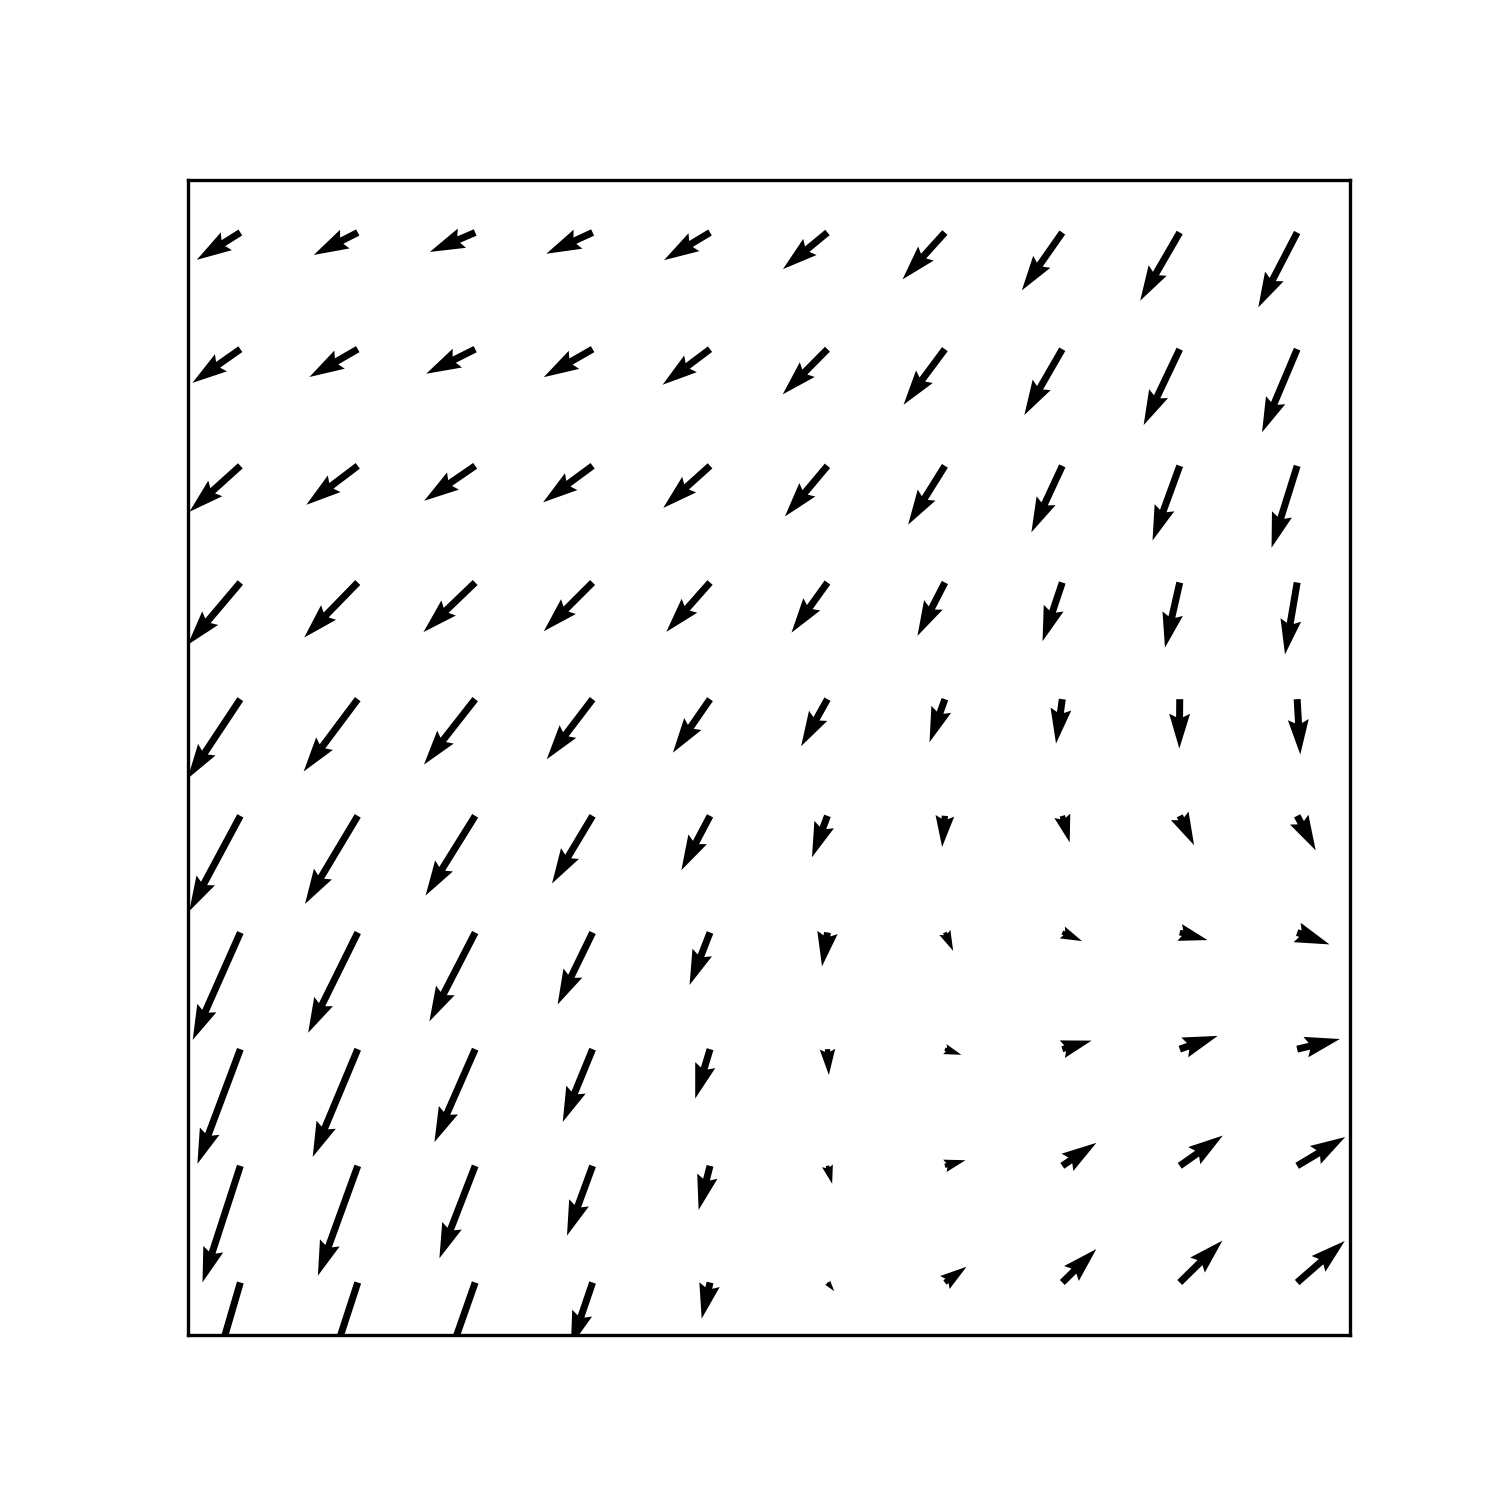
\includegraphics[keepaspectratio]{kernel_example_direction_var.png}}

\subcaption{\label{}Invariant Kernel Direction}
\end{minipage}%
%
\begin{minipage}{0.50\linewidth}

\pandocbounded{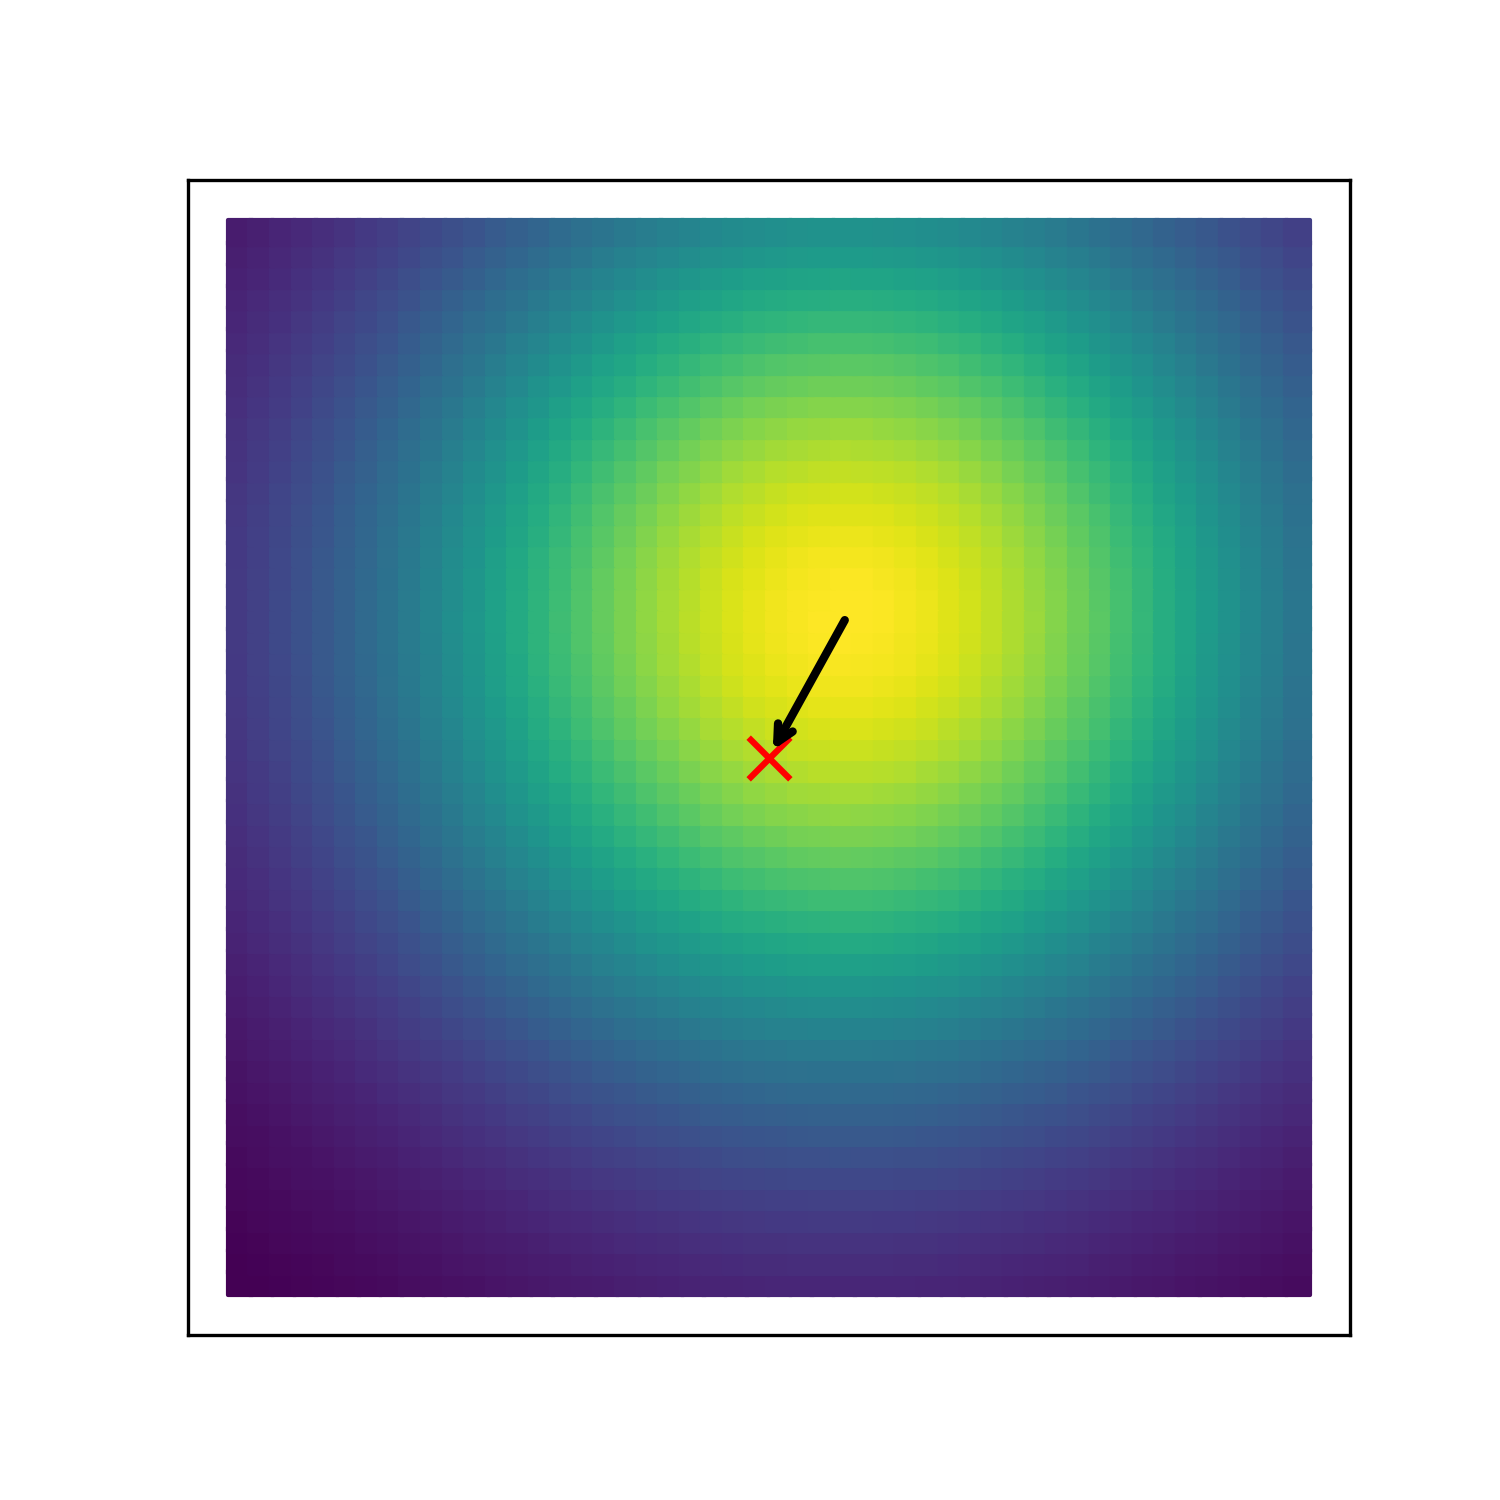
\includegraphics[keepaspectratio]{kernel_example_strength_var.png}}

\subcaption{\label{}Invariant Kernel Strength}
\end{minipage}%

\caption{\label{fig-examplekernelvar}A spatially invarient kernel across
the region \([0,1]\times[0,1]\). The kernel direction is shown on the
left, and on the right is the amount that each point affects the point
\((0.5,0.5)\), marked with a red cross. `Flow' is allowed to vary by a
function \(\bv m(\bv s)\) which is chosen randomly using a basis
expansion (see Section~\ref{sec-kerneldecomp}). The other two parameters
are set at \(a=150,b=0.2\).}

\end{figure}%

\chapter{Spectral Representations}\label{spectral-representations}

The key to being able to computationally work with IDEMs, as perhaps
originally made by Wikle and Cressie (1999), is to work with the
spectral decomposition of the process, in order to coerce the model
heirarchy into a more familiar linear dynamical system form, like
Equation~\ref{eq-ldstm}.

This kind of dimension-reduction allows us to parameterise spatial
fields with as few or as many parameters as we want.

\section{Process decomposition}\label{process-decomposition}

Choose a complete class of spatial spectral basis functions,
\(\phi_i(\bv s)\), and decompose the process spatial field at each time;

\begin{equation}\phantomsection\label{eq-processdecomp}{\begin{split}
Y_t(\bv s) \approx \sum_{i=1}^{r} \alpha_{i,t} \phi_i(\bv s), \quad t=0,\dots,T.
\end{split}
}\end{equation}

where we truncate the expansion at some \(r\in\mathbb N\). Notice that
we can write this in vector/matrix form; considering times
\(t=1,2,\dots, T\), we set

\begin{equation}\phantomsection\label{eq-vecmats}{\begin{split}
\bv \phi(\bv s) &= (\phi_1(\bv s), \phi_2(\bv s), \dots, \phi_r(\bv s))^{\intercal},\\
\bv \alpha_t &= (\alpha_{1,t}, \alpha_{2,t}, \dots, \alpha_{r, t})^{\intercal}.
\end{split}
}\end{equation}

Now, (Equation~\ref{eq-processdecomp}) gives us

\begin{equation}\phantomsection\label{eq-pbvec}{\begin{split}
Y(\bv s; t) \approx \bv \phi^{\intercal}(\bv s)  \alpha(t).\\
\end{split}
}\end{equation}

We can effectively now work exclusively with \(\bv alpha_t\). To do so,
we need to find the evolution equation of \(\bv alpha_t\), as given
below.

\begin{theorem}[Spectral form of the state
evolution]\protect\hypertarget{thm-state_form}{}\label{thm-state_form}

Define the \emph{Gram matrix};

\begin{equation}\phantomsection\label{eq-gram}{\Psi \coloneq \int_{\mathcal D_s} \bv \phi(\bv s) \bv \phi(\bv s)^\intercal d\bv s.
}\end{equation}

Then, the basis coefficients evolve by the equation

\begin{equation}\phantomsection\label{eq-stateev}{\bv \alpha_{t+1} = M \bv\alpha_t + \bv\eta_t,
}\end{equation}

where
\(M = \Psi^{-1} \int\int \bv\phi(\bv s) \kappa(\bv s, \bv r)\bv\phi(\bv r)^\intercal d\bv r d \bv s\)
and \(\bv\eta_t =\Psi^{-1} \int \bv \phi(\bv s)\omega_t(s)d\bv s\).

\end{theorem}

\begin{proof}
(Adapting from Dewar, Scerri, and Kadirkamanathan 2008), write out the
process equation, (Equation~\ref{eq-IDEM}), using the first equation of
(Equation~\ref{eq-pbvec});

\[Y_{t+1}(\bv s) = \bv \phi(\bv s)^{\intercal} \alpha_{t+1} = \int_{\mathcal D_s} \kappa(\bv s, \bv r) \bv\phi(\bv r)^{\intercal}\bv \alpha_t d\bv r + \omega_t(\bv s),
\]

We then multiply both sides by \(\bv \phi(s)\) and integrate over
\(\bv s\)

\[\begin{split}
\int_{\mathcal D_s} \bv\phi(\bv s)\bv\phi(\bv s)^{\intercal} d\bv s \bv\alpha_{t+1} &= \int\bv\phi(\bv s)\int \kappa(\bv s, \bv r)\bv\phi(\bv r)^\intercal d\bv r  d \bv s\ \bv\alpha_t + \int \bv \phi(\bv s)\omega_t(s)d\bv s\\
\Psi \bv\alpha_{t+1} &= \int\int \bv\phi(\bv s)\kappa(\bv s, \bv r) \bv\phi(\bv r)^\intercal d\bv r d \bv s\ \bv\alpha_t + \int \bv \phi(\bv s)\omega_t(s)d\bv s.
\end{split}
\]

So, finally, pre-multipling by the inverse of the gram matrix,
\(\Psi^{-1}\) (Equation~\ref{eq-gram}), we arrive at the result. \qed
\end{proof}

\section{Spectral form of the Process
Noise}\label{spectral-form-of-the-process-noise}

We still have to set out what the process noise, \(\omega_t(\bv s)\),
and it's spectral couterpart, \(\bv \eta_t\), are. Dewar, Scerri, and
Kadirkamanathan (2008) fix the variance of \(\omega_t(\bv s)\) to be
uniform and uncorrelated across space and time, with
\(\omega_t(\bv s) \sim \mathcal N(0,\sigma^2)\) It is then easily shown
that \(\bv\eta_t\) is also normal, with
\(\bv\eta_t \sim \mathcal N(0, \sigma^2\Psi^{-1})\).

However, in practice, we simulate in the spectral domain; that is, if we
want to keep things simple, it would make sense to specify (and fit) the
distribution of \(\bv\eta_t\), and compute the variance of
\(\omega_t(\bv s)\) if needed.

\begin{lemma}[]\protect\hypertarget{lem-omegadist}{}\label{lem-omegadist}

Let \(\bv\eta_t \sim \mathcal N(0, \Sigma_\eta)\), and
\(\cov[\bv\eta_t, \bv \eta_{t+\tau}] =0\), \(\forall \tau>0\). Then
\(\omega_t(\bv s)\) has covariance

\[\cov [\omega_t(\bv s), \omega_{t+\tau}(\bv r)] = \begin{cases}
\bv\phi(\bv s)^\intercal \Sigma_\eta \bv\phi(\bv r) & \text{if }\tau=0\\
0 & \text{else}\\
\end{cases}
\]

\end{lemma}

\begin{proof}
Consider \(\Psi \bv\eta_t\), and consider the case \(\tau=0\). It is
clearly normal, with zero expectation and variance (using
Equation~\ref{eq-gram}),

\begin{equation}\phantomsection\label{eq-var1}{\begin{split}
\var[\Psi \bv\eta_t] &= \Psi \var[\bv\eta_t] \Psi^\intercal = \Psi\Sigma_\eta\Psi^\intercal,\\
&= \int_{\mathcal D_s} \bv\phi(\bv s) \bv\phi(\bv s)^\intercal d\bv s \  \Sigma_\eta \ \int_{\mathcal D_s} \bv\phi(\bv r) \bv\phi(\bv r)^\intercal d\bv r\\
&=  \int\int_{\mathcal D_s^2} \bv\phi(\bv s) \bv\phi(\bv s)^\intercal \  \Sigma_\eta \  \bv\phi(\bv r) \bv\phi(\bv r)^\intercal d\bv r d\bv s\\
\end{split}
}\end{equation}

Since it has zero expectation, we also have

\begin{equation}\phantomsection\label{eq-var2}{\begin{split}
\var[\Psi\bv\eta_t] &= \mathbb E[(\Psi\bv\eta_t) (\Psi\bv\eta_t)^\intercal] = \mathbb E[\Psi\bv\eta_t\bv\eta_t^\intercal\Psi^\intercal]\\
&= \mathbb E \left[ \int_{\mathcal D_s} \bv\phi(\bv s)\omega_t(\bv s)d\bv s \int_{\mathcal D_s} \bv \phi(\bv r)^\intercal \omega_t(\bv r) d\bv r \right]\\
&= \int\int_{\mathcal D_s^2} \bv\phi(\bv s)\  \mathbb E[\omega_t(\bv s)\omega_t(\bv r)]\  \bv \phi(\bv r)^\intercal d\bv s d \bv r.
\end{split} 
}\end{equation}

We can see that, comparing (Equation~\ref{eq-var1}) and
(Equation~\ref{eq-var2}), we have

\[\cov [\omega_t(\bv s), \omega_t(\bv r)] = \mathbb E[\omega_t(\bv s)\omega_t(\bv r)]= \bv\phi(\bv s)^\intercal \Sigma_\eta \bv\phi(\bv r).
\]

Since, once again, \(\mathbb E[\bv\omega_t(\bv s)]=0\).

For the \(\tau\neq0\) case, it is simple to show that the covariance is
0.

\qed
\end{proof}

\section{Kernel Parameterisations}\label{sec-kerneldecomp}

Next is the part of the system, which defines the dynamics; the kernelf
function, \(\kappa\). There are a few ways to handle the kernel. One of
the most obvious is to expand it out into a spectral decomposition as
well;

\[\kappa \approx \sum_i \beta_i\psi(\bv s, \bv r).
\]

This can allow for a wide range of interestingly shaped kernel
functions, but see how these basis functions must now act on
\(\mathbb R^2\times \mathbb R^2\); to get a wide enough space of
possible functions, we would likely need many terms in the spectral
expansion.

A much simpler approach would be to simply parameterise the kernel
function, to \(\kappa(\bv s, \bv r, \bv \theta_\kappa)\). We then
establish a simple shape for the kernel (e.g.~Gaussian) and rely on very
few parameters (for example, scale, shape, offsets). The example kernel
used in the \texttt{jaxidem} is a Gaussian-shape kernel;

\[\kappa(\bv s, \bv r; \bv m, a, b) = a \exp \left( -\frac{1}{b} \vert \bv s- \bv r +\bv m\vert^2 \right). 
\]

Of course, this kernel lacks spatial dependance. We can add spatial
variance back by adding dependance on \(\bv s\) to the parameters, for
example, variyng the offset term as \(\bv m(\bv s)\). Of course, now we
are back to having entire functions as parameters, but taking the
spectral decomposition of the parameters we actually want to be
spatially variant seems like a reasonable middle ground (Cressie and
Wikle 2015). The actual parameters of such a spatially-variant kernel
are then the spectral coefficients for the expansion of any spatially
variant parameters, as well as any constant parameters. This is
precisely what is plotting in Figure~\ref{fig-examplekernelvar}, where
the spectral coeficients are randomly sampled from a multivariate normal
distribution;

\[\begin{split}
  \bv m(\bv s) = \left(\begin{matrix}
    \sum_{i=1}^{r_m} \phi_{\kappa,i}(\bv s) m^{(x)}_i\\
    \sum_{i=1}^{r_m} \phi_{\kappa,i}(\bv s) m^{(y)}_i
  \end{matrix}\right),
\end{split}
\]

where \(m^{(x)}_i\) and \(m^{(y)}_i\) are coefficients for the x and y
coordinates respectively, and \(\phi_{\kappa, i}(\bv s)\) are basis
functions (e.g.~bisquare functions in
Figure~\ref{fig-examplekernelvar}).

\section{IDEM as a linear dynamical
system}\label{idem-as-a-linear-dynamical-system}

To summarise, we have taken a truncated spectral decompostion to write
the Integro-difference equation model as a more traditional linear
dynamical system form (Equation~\ref{eq-stateev}). All that is left is
to include our observations in our system.

Lets assume that at each time \(t\) there are \(n_t\) observations at
locations \(\bv s_{1,t},\dots, \bv s_{n_{t},t}\). We write the vector of
the process at these points as
\(\bv Y(t) = (Y(s_{1,t};t), \dots, Y(s_{n_{t},t};t))^\intercal\), and,
in it's expanded form \(\bv Y_t = \Phi_t \bv\alpha_t\), where
\(\Phi \in \mathbb R^{r\times n_{t}}\) is

\[\begin{split}
\{\Phi_{t}\}_{i, j} = \phi_{i}(s_{j,t}).
\end{split}
\]

For the covariates, we write the matrix
\(X_t = (\bv X(\bv s_{1, t}), \dots, \bv X(\bv s_{1=n_{t}, t})^\intercal\).
We then have

\[\begin{split}
\bv Z_t &= \Phi \alpha_t + X_{t} \bv \beta + \bv \epsilon_t, \quad t = 1,\dots, T,\\
\bv \alpha_{t+1} &= M\bv \alpha_t + \bv\eta_t,\quad t = 0,2,\dots, T-1,\\
M &= \int_{\mathcal D_s}\bv\phi(\bv s) \bv\phi(\bv s)^\intercal d\bv s \int_{\mathcal D_s^2}\bv\phi(\bv s) \kappa(\bv s, \bv r; \bv\theta_\kappa)\bv\phi(\bv r)^\intercal d\bv r d \bv s,
\end{split}
\]

Writing \(\tilde{\bv{Z}}_t = \bv Z_t - X_t \bv \beta\),

\begin{equation}\phantomsection\label{eq-stateidem}{\begin{split}
\tilde{\bv Z}_t &= \Phi_{t} \bv \alpha_t + \bv \epsilon_t,\quad &t = 1,2,\dots, T,\\
\bv \alpha_{t+1} &= M \bv \alpha_t + \bv\eta_t,\quad &t = 0,1, \dots, T.\\
\end{split}
}\end{equation}

We should also initialise
\(\bv \alpha_0 \sim \mathcal N^{r}(\bv m_{0}, \Sigma_{0})\), and fix
simple distrubtions to the noise terms,

\[\begin{split}
\epsilon_{t,i} \overset{\mathrm{iid}}{\sim} \mathcal N(0,\sigma^2_\epsilon),\\
\eta_{t,i} \overset{\mathrm{iid}}{\sim} \mathcal N(0,\sigma^2_\eta),
\end{split}
\]

which are (also) independant in time.

As in, for example, (Wikle and Cressie 1999),
Equation~\ref{eq-stateidem} is now in a traditional enough form that the
Kalman filter can be applied to filter and compute many necessary
quantities for inference, including the marginal likelihood. We can use
these quantities in either an EM algorithm or a Bayesian approach, or
directly maximise the marginal data likelihood

We now move on to an example simulation of this kind of model using it's
spectral decomposition and \texttt{jaxidem}.

\section{Example Simulation}\label{example-simulation}

We can now use the above to simulate easily from such models; once we
have chosen the appropriate decompositions, we simply compute \(M\) and
propegate \(\bv \alpha_t\) as we would when simulating any other linear
dynamic system. We then use the spectral coefficients to generate
\(Y_t(\bv s)\) and \(Z_t(\bv s)\) in the obvious way.

\texttt{jaxidem} implements this in the function \texttt{simIDEM}, or
through the more user-friendly method \texttt{idem.idemModel.simulate}.
An object of the idemModel class contains all the necesary information
about basis decompositions, and the simulate methods calls
\texttt{simIDEM} without comprimising its jit-ability (although
just-in-time computation obviously isn't as important for simulation,
the jit-ed function could save compile time if someone want to simulate
from many models).

The \texttt{gen\_example\_idem} method creates a simple IDEM object
without many required parameters;

\begin{Shaded}
\begin{Highlighting}[]
\NormalTok{key }\OperatorTok{=}\NormalTok{ jax.random.PRNGKey(}\DecValTok{1}\NormalTok{)}
\NormalTok{keys }\OperatorTok{=}\NormalTok{ rand.split(key, }\DecValTok{2}\NormalTok{)}

\NormalTok{model }\OperatorTok{=}\NormalTok{ idem.gen\_example\_idem(keys[}\DecValTok{0}\NormalTok{], k\_spat\_inv}\OperatorTok{=}\VariableTok{False}\NormalTok{)}

\NormalTok{process\_data, obs\_data }\OperatorTok{=}\NormalTok{ model.simulate(keys[}\DecValTok{1}\NormalTok{], T}\OperatorTok{=}\DecValTok{3}\NormalTok{, nobs}\OperatorTok{=}\DecValTok{50}\NormalTok{)}
\end{Highlighting}
\end{Shaded}

The resulting objects are of class \texttt{st\_data}, containing a
couple of niceties for handling spatio-temporal data, while still
storing all data as JAX arrays. For example, the \texttt{show\_plot},
\texttt{save\_plot} and \texttt{save\_gif} methods provide easy
plotting;

\begin{Shaded}
\begin{Highlighting}[]
\NormalTok{process\_data.save\_plot(}\StringTok{\textquotesingle{}process\_data\_example.png\textquotesingle{}}\NormalTok{)}
\NormalTok{obs\_data.save\_plot(}\StringTok{\textquotesingle{}obs\_data\_example.png\textquotesingle{}}\NormalTok{)}
\end{Highlighting}
\end{Shaded}

\begin{figure}[h]

\begin{minipage}{\linewidth}

\pandocbounded{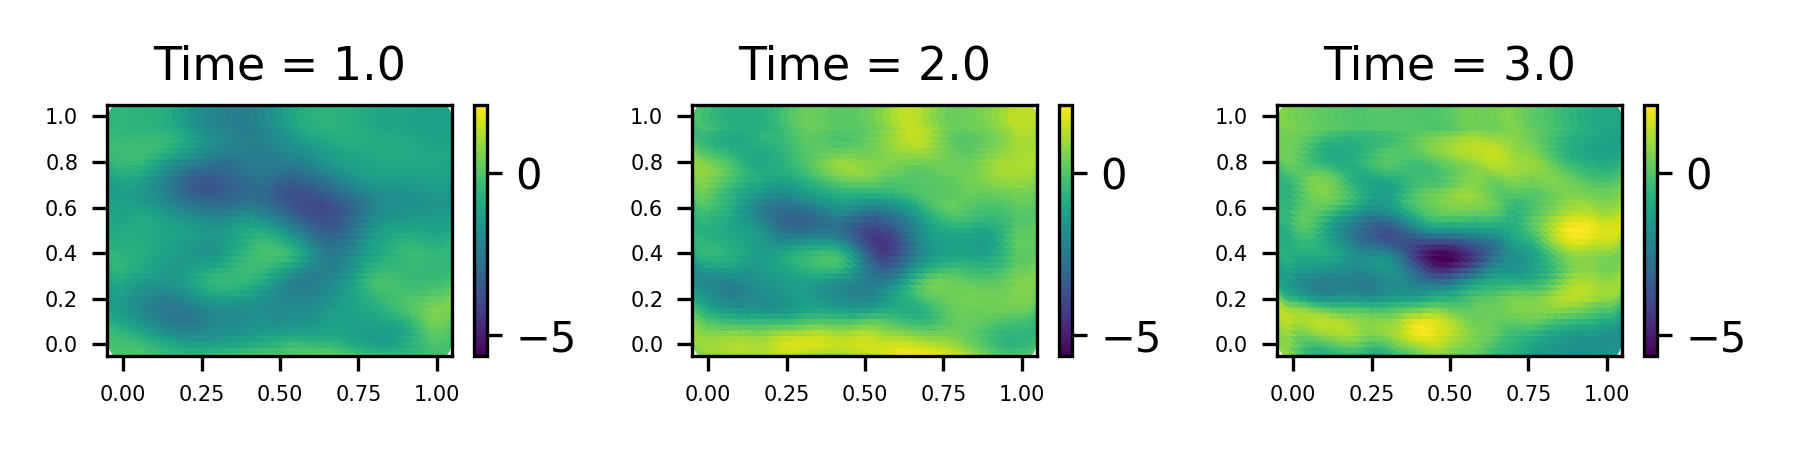
\includegraphics[keepaspectratio]{process_data_example.png}}

\subcaption{\label{}Process Simulation}
\end{minipage}%
\newline
\begin{minipage}{\linewidth}

\pandocbounded{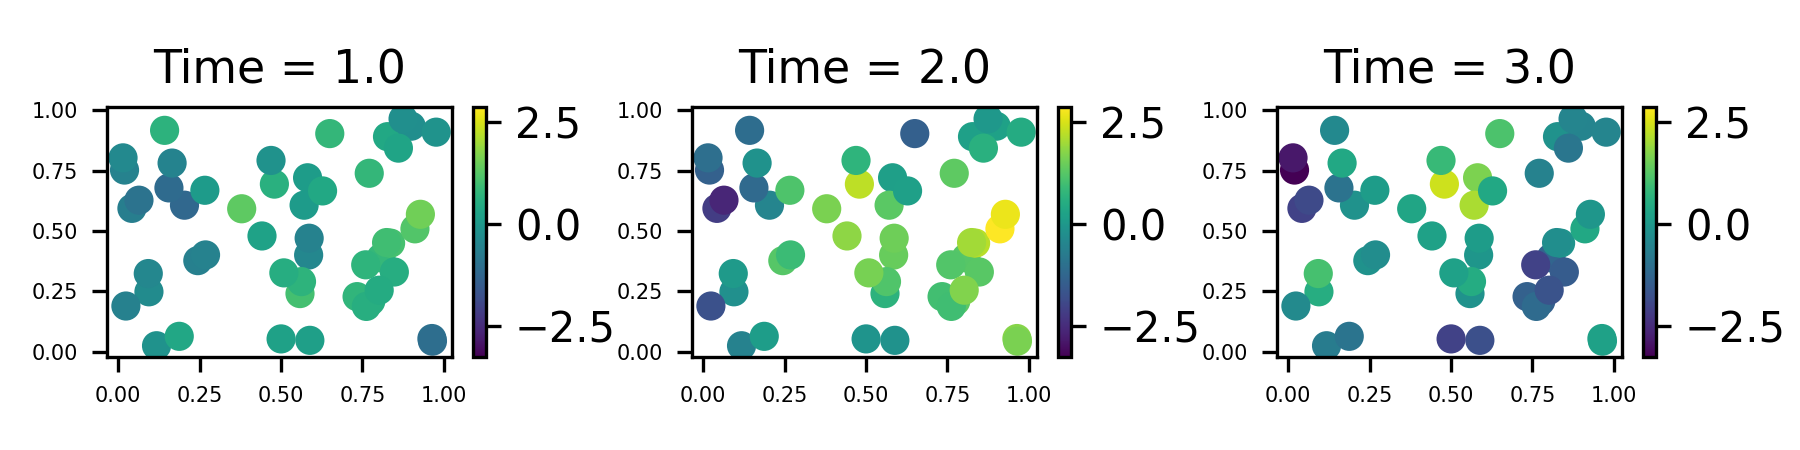
\includegraphics[keepaspectratio]{obs_data_example.png}}

\subcaption{\label{}Observation Simulation}
\end{minipage}%

\caption{\label{fig-examplesim}Example simulations from an
Integro-difference Equation Model. Kernel is generated with spatially
varying flow terms, generated by bisquare basis functions with randomly
generated coefficient. Not that some artifacts from the decomposition
are visible, such as a faint checkerboard pattern in the process.}

\end{figure}%

\chapter{Filtering, Forecasting and Maximum Likelihood
Estimation}\label{filtering-forecasting-and-maximum-likelihood-estimation}

The Kalman filter gives us linear estimates for the distribution of
\(\bv\alpha_r\mid \{\bv Z_t=\bv z_t\}_{t=0,...,r}\) in any dynamical
system like Equation~\ref{eq-ldstm}. For full discussions and proofs of
the Kalman filter, see, for example, (Shumway, Stoffer, and Stoffer
2000).

\section{The Kalman Filter}\label{sec-kalmanfilter}

Firstly, we should establish some notation. Write

\[\begin{split}
m_{i \mid j} &= \mathbb E[\bv\alpha_i \mid \{\bv Z_t=\bv z_t\}_{t=0,\dots,j}],\\
P_{i \mid j} &= \var[\bv\alpha_i \mid \{\bv Z_t=\bv z_t\}_{t=0,\dots,j}],\\
P_{i,j \mid k} &= \cov[\bv\alpha_i, \bv\alpha_k \mid \{\bv Z_t=\bv z_t\}_{t=0,\dots,k}].
\end{split}
\]

For the initial terms, we choose bayesian-like prior moments
\(m_{0\mid0}=m_0\) and \(P_{0\mid0}=\Sigma_0\). For convenience and
generality, we write \(\Sigma_\eta\) and \(\Sigma_\epsilon\) for the
variance matrices of the process and observations. Note that, if the
number of observations change at each time point (for example, due to
missing data), then \(\Sigma_\epsilon\) should be time variyng; we could
either always keep it as uncorrelated so that
\(\Sigma_\epsilon = \mathrm{diag} (\sigma_\epsilon^2)\), or perhaps put
some kind of distance-dependant covariance function to it.

To move the filter forward, that is, given \(m_{t\mid t}\) and
\(P_{t\mid t}\), to get \(m_{t+1\mid t+1}\) and \(P_{t+1\mid t+1}\), we
first \emph{predict}

\begin{equation}\phantomsection\label{eq-kalman-predict}{\begin{split}
\bv m_{t+1\mid t} &= M \bv m_{t\mid t},\\
P_{t+1\mid t} &= M P_{t\mid t} M^\intercal + \Sigma_\eta,
\end{split}
}\end{equation}

then we add our new information, \(z_{t}\);

\begin{equation}\phantomsection\label{eq-kalman-update}{\begin{split}
\bv m_{t+1\mid t+1} &= \bv m_{t+1\mid t} + K_{t+1} \bv e_{t+1}\\
P_{t+1\mid t+1} &= [I- K_{t+1}\Phi_{t+1}]P_{t+1\mid t}
\end{split} 
}\end{equation}

where \(K_{t+1}\) is the \emph{Kalman gain};

\[\begin{split}
K_{t+1} = P_{t+1\mid t}\Phi_{t+1}^\intercal [\Phi_{t+1} P_{t+1\mid t} \Phi_{t+1}^\intercal + \Sigma_\epsilon]^{-1}, \quad t=0,\dots,T-1
\end{split}
\]

and \(\bv e_{t+1}\) are the \emph{prediction errors}

\[\begin{split}
\bv e_{t+1} = \tilde{\bv z}_{t+1}-\Phi_{t+1} \bv m_{t+1\mid t}, \quad t=1,\dots,T 
\end{split}
\]

Starting with \(m_0\) and \(P_0\), we can then iteratively move across
the data to eventually compute \(m_{T\mid T}\) and \(P_{T\mid T}\).

Assuming Gaussian all random variables here are Guassian, this is the
optimal mean-square estimators for these quantities, but even outside of
the Gaussian case, these are optimal for the class of \emph{linear}
operators.

We can compute the marginal data likelihood alongside the kalman fiter
using the prediciton errors \(\bv e_t\). These, under the assumptions we
have made about \(\bv \eta_t\) and \(\bv\epsilon_t\) being normal, are
also normal with zero mean and variance

\[\begin{split}
\mathbb V\mathrm{ar}[\bv e_t]=\Sigma_t= \Phi_{t} P_{t\mid t-1} \Phi_{t}^\intercal + \Sigma_\epsilon. 
\end{split}
\]

Therefore, the log-likelihood at each time is

\[\begin{split}
\mathcal L(Z\mid\bv\theta) = -\frac12\sum \log\det(\Sigma_t(\bv\theta)) - \frac12 \sum\bv e_t(\bv\theta)^\intercal\Sigma_{t}(\bv\theta)^{-1} \bv e_t(\bv\theta) - \frac{n_{t}}{2}\log(2*\pi).
\end{split}
\]

Summing these across time, we get the log likelihood for all the data.

A simplified example of the kalman filter function, written to be jax
compatible, used in the package is this;

\newpage
\small

\begin{Shaded}
\begin{Highlighting}[]
\AttributeTok{@jax.jit}
\KeywordTok{def}\NormalTok{ kalman\_filter(m\_, P\_0, M, PHI\_obs, Sigma\_eta, Sigma\_eps, ztildes):}
\NormalTok{    nbasis }\OperatorTok{=}\NormalTok{ m\_0.shape[}\DecValTok{0}\NormalTok{]}
\NormalTok{    nobs }\OperatorTok{=}\NormalTok{ ztildes.shape[}\DecValTok{0}\NormalTok{]}

    \AttributeTok{@jax.jit}
    \KeywordTok{def}\NormalTok{ step(carry, z\_t):}
\NormalTok{        m\_tt, P\_tt, \_, \_, ll, \_ }\OperatorTok{=}\NormalTok{ carry}

        \CommentTok{\# predict}
\NormalTok{        m\_pred }\OperatorTok{=}\NormalTok{ M }\OperatorTok{@}\NormalTok{ m\_tt}
\NormalTok{        P\_pred }\OperatorTok{=}\NormalTok{ M }\OperatorTok{@}\NormalTok{ P\_tt }\OperatorTok{@}\NormalTok{ M.T }\OperatorTok{+}\NormalTok{ Sigma\_eta}

        \CommentTok{\# Update}
        \CommentTok{\# Prediction Errors}
\NormalTok{        eps\_t }\OperatorTok{=}\NormalTok{ z\_t }\OperatorTok{{-}}\NormalTok{ PHI\_obs }\OperatorTok{@}\NormalTok{ m\_pred}

\NormalTok{        Sigma\_t }\OperatorTok{=}\NormalTok{ PHI\_obs }\OperatorTok{@}\NormalTok{ P\_pred }\OperatorTok{@}\NormalTok{ PHI\_obs.T }\OperatorTok{+}\NormalTok{ Sigma\_eps}
        \CommentTok{\# Kalman Gain}
\NormalTok{        K\_t }\OperatorTok{=}\NormalTok{ (jnp.linalg.solve(Sigma\_t, PHI\_obs)}\OperatorTok{@}\NormalTok{ P\_pred.T).T}

\NormalTok{        m\_up }\OperatorTok{=}\NormalTok{ m\_pred }\OperatorTok{+}\NormalTok{ K\_t }\OperatorTok{@}\NormalTok{ eps\_t}
\NormalTok{        P\_up }\OperatorTok{=}\NormalTok{ (jnp.eye(nbasis) }\OperatorTok{{-}}\NormalTok{ K\_t }\OperatorTok{@}\NormalTok{ PHI\_obs) }\OperatorTok{@}\NormalTok{ P\_pred}

        \CommentTok{\# likelihood of epsilon, using cholesky decomposition}
\NormalTok{        ll\_new }\OperatorTok{=}\NormalTok{ ll }\OperatorTok{{-}} \FloatTok{0.5} \OperatorTok{*}\NormalTok{ n }\OperatorTok{*}\NormalTok{ jnp.log(}\DecValTok{2}\OperatorTok{*}\NormalTok{jnp.pi) }\OperatorTok{{-}} \OperatorTok{\textbackslash{}}
            \FloatTok{0.5} \OperatorTok{*}\NormalTok{ jnp.log(jnp.linalg.det(Sigma\_t)) }\OperatorTok{{-}\textbackslash{}}
            \FloatTok{0.5} \OperatorTok{*}\NormalTok{ e.T }\OperatorTok{@}\NormalTok{ jnp.linalg.solve(Sigma\_t, e)}

        \ControlFlowTok{return}\NormalTok{ (m\_up, P\_up, m\_pred, P\_pred, ll\_new, K\_t), (m\_up, P\_up, m\_pred, P\_pred, ll\_new, K\_t,)}

\NormalTok{    carry, seq }\OperatorTok{=}\NormalTok{ jl.scan(}
\NormalTok{        step,}
\NormalTok{        (m\_0, P\_0, m\_0, P\_0, }\DecValTok{0}\NormalTok{, jnp.zeros((nbasis, nobs))),}
\NormalTok{        ztildes.T,}
\NormalTok{    )}

    \ControlFlowTok{return}\NormalTok{ (carry[}\DecValTok{4}\NormalTok{], seq[}\DecValTok{0}\NormalTok{], seq[}\DecValTok{1}\NormalTok{], seq[}\DecValTok{2}\NormalTok{][}\DecValTok{1}\NormalTok{:], seq[}\DecValTok{3}\NormalTok{][}\DecValTok{1}\NormalTok{:], seq[}\DecValTok{5}\NormalTok{][}\DecValTok{1}\NormalTok{:])}
\end{Highlighting}
\end{Shaded}

\normalsize

For the documentation of the method proveded by the package, see {[}WORK
OUT HOW TO LINK DO PAGES{]}

\section{The Information Filter}\label{the-information-filter}

In some computational scenarios, it is beneficial to work with vectors
of consistent dimension. In Python JAX, the efficient \texttt{scan}
method works only with such arrays; JAX has no support for jagged
arrays, and traditional for loops will likely lead to long compile times
when jit-compiled. Although there are some tools in JAX to get around
this problem (namely the \texttt{jax.tree} functions which allow mapping
over PyTrees), scan is still a large problem; since the Kalman filter
is, at it's core, a scan-type operation (scanning over the data), this
causes a large problem when the observation dimension is changing, as is
frequent with many spatio-temporal data.

But it is possible to re-write the Kalman filter in a way which is
compatible with this kind of data. The `information filter' (sometimes
called inverse Kalman filter or other names) involves transforming the
data into its `information form', which will always have consistent
dimension, allowing us to avoid jagged scans.

The information filter is simply the Kalman filter re-written to use the
Gaussian distribution's canonical parameters \footnote{that is, the
  parameters of the Gaussian distribution in it's exponential family
  form}, those being the information vector and the information matrix.
If a Gaussian distribution has mean \(\bv\mu\) and variance matrix
\(\Sigma\), then the corresponding \emph{information vector} and
\emph{information matrix} is \(\nu = \Sigma^{-1}\mu\) and
\(Q = \Sigma^{-1}\), correspondingly.

\begin{theorem}[The Information
Filter]\protect\hypertarget{thm-information_filter}{}\label{thm-information_filter}

The Kalman filter can be rewritten in information form as follows (for
example, Khan 2005). Write

\[\begin{split}
Q_{i\mid j} &= P_{i\mid j}\\
\bv\nu_{i\mid j} &= Q_{i\mid j} \bv m_{i\mid j}
\end{split}
\]

and transform the observations into their `information form', for
\(t=1,\dots, T\)

\begin{equation}\phantomsection\label{eq-obsinfo}{\begin{split}
I_{t} = \Phi_{t}^{\intercal} \Sigma_{\epsilon}^{-1}\Phi_{t},\\
i_{t} = \Phi_{t}^{\intercal} \Sigma_{\epsilon}^{-1} \bv z_{t}.
\end{split}
}\end{equation}

The prediction step now becomes

\[\begin{split}
\bv\nu_{t+1\mid t} &= (I-J_t) M^{-1}\bv\nu_{t\mid t}\\
Q_{t+1\mid t} &= (I-J_t) S_{t} 
\end{split}
\]

where \(S_t = M^{-\intercal} Q_{t\mid t} M^{-1}\) and
\(J_t = S_t [S_{t}+\Sigma_{\eta}^{-1}]^{-1}\).

Updating is now as simple as adding the information-form observations;

\[\begin{split}
  \bv\nu_{t+1\mid t+1} &= \bv\nu_{t+1\mid t} + i_{t+1}\\
  Q_{t+1\mid t+1} &= Q_{t+1\mid t} + I_{t+1}.
\end{split}
\]

\end{theorem}

Proof in Appendix (Section~\ref{sec-app1}.)

We can see that the information form of the observations
(Equation~\ref{eq-obsinfo}) will always have the same dimension
\footnote{that being the process dimension, previously labelled \(r\),
  the number of basis functions used in the expansion of the process}.
For our purposes, this means that \texttt{jax.lax.scan} will work after
we `informationify' the data, which can be done using
\texttt{jax.tree.map}. This is implemented in the functions
\texttt{information\_filter} and \texttt{information\_filter\_indep}
(for uncorrelated errors).

There are other often cited advantages to filtering in this form. It can
be quicker that the traditional form in certain cases, especially when
the observation dimension is bigger than the state dimension (since you
solve a smaller system of equations with \([S_t + \Sigma_\eta]^{-1}\) in
the process dimension instead of
\([\Phi_t P_{t+1\mid t} \Phi_t^\intercal + \Sigma_\epsilon]^{-1}\) in
the observation dimension) (Assimakis, Adam, and Douladiris 2012).

The other often mentioned advantage is the ability to use a flat prior
for \(\alpha_0\); that is, we can set \(Q_0\) as the zero matrix,
without worriying about an infinite variance matrix. While this is
indeed true, it is actually possible to do the same with the Kalman
filter by doing the first step analytically, see
Section~\ref{sec-vagueprior}.

As with the kalman filter, it is also possible to get the data
likelihood in-line as well. Again, we would like to stick with things in
the state dimension, so working direclty with the prediction errors
\(\bv e_t\) should be avoided. Luckily, by multipliying the errors by
\(\Phi_t^\intercal \Sigma_\epsilon^{-1}\), we can define the
`information errors' \(\bv \iota_t\);

\[\begin{split}
  \bv \iota_t &= \Phi_t^\intercal \Sigma_\epsilon^{-1} \bv e_t = \Phi_t^\intercal \Sigma_\epsilon^{-1} \tilde{\bv z}_t -\Phi_t^\intercal \Sigma_\epsilon^{-1}\Phi_t m_{t\mid t-1}\\
  &= i_t - I_tQ_{t\mid t-1}^{-1}\bv \nu_{t\mid t-1}.
\end{split}
\]

The variance of this quantity is also easy to find;

\[\begin{split}
  \var[\bv \iota_t] &= \Phi_t^\intercal \Sigma_\epsilon^{-1}\var[\bv e_t]\Sigma_\epsilon^{-1}\Phi_t\\
  &= \Phi_t^\intercal \Sigma_\epsilon^{-1} [\Phi_{t} P_{t\mid t-1} \Phi_{t}^\intercal + \Sigma_\epsilon] \Sigma_\epsilon^{-1}\Phi_t\\
  &= \Phi_t^\intercal \Sigma_\epsilon^{-1}\Phi_{t} Q_{t\mid t-1}^{-1} \Phi_{t}^\intercal \Sigma_\epsilon^{-1}\Phi_t \Phi_t^\intercal \Sigma_\epsilon^{-1} \Phi_t\\
  &= I_t Q_{t\mid t-1}^{-1} I_t^\intercal + I_t =: \Sigma_{\iota, t}.
\end{split}
\]

Noting that \(\bv \iota\) clearly still has mean zero, this allows us
once again to compute the log likelihood, this time through \(\bv\iota\)

\[\begin{split}
\mathcal L(z_t\mid\bv\theta) = -\frac12\sum \log\det(\Sigma_{\iota, t}(\bv\theta)) - \frac12 \sum\bv \iota_t(\bv\theta)^\intercal\Sigma_{\iota, t}(\bv\theta)^{-1} \bv \iota_t(\bv\theta) - \frac{r}{2}\log(2*\pi).
\end{split}
\]

\section{Smoothing}\label{smoothing}

Beyond the filtering, another task is \emph{smoothing}. That is, filters
estimate \(\bv m_{T\mid T}\) and \(P_{T\mid T}\), but there is use for
estimating \(\bv m_{t\mid T}\) and \(P_{t\mid T}\) for all
\(t=0,\dots, T\).

We simply work backwards from \(\bv m_{T\mid T}\) and \(P_{T\mid T}\)
values using what is known as the \emph{Rauch-Tung-Striebel (RTS)
smoother};

\begin{equation}\phantomsection\label{eq-kalmansmooth}{\begin{split}
\bv m_{t-1\mid T} &= \bv m_{t-1\mid t-1} + J_{t-1}(\bv m_{t\mid T} - \bv m_{t\mid t-1}),\\
P_{t-1\mid T} &= P_{t-1\mid t-1} + J_{t-1}(P_{t\mid T} - P_{t\mid t-1})J_{t-1}^\intercal,
\end{split}
}\end{equation}

where,

\[\begin{split}
J_{t-1} = P_{t-1\mid t-1}M^\intercal[P_{t\mid t-1}]^{-1}.
\end{split}
\]

We can clearly see, then, that it is crucial to keep the values in
Equation~\ref{eq-kalman-predict}.

We can then also compute the lag-one cross-covariance matrices
\(P_{t,t-1\mid T}\) using the \emph{Lag-One Covariance Smoother}. This
will b useful, for example, in the expectation-maximisation algorithm
later. From

\[\begin{split}
P_{T,T-1\mid T} = (I - K_T\Phi_{T}) MP_{T-1\mid T-1},
\end{split}
\]

we can compute the lag-one covariances

\begin{equation}\phantomsection\label{eq-lag1smooth}{\begin{split}
P_{t, t-1\mid T} = P_{t\mid t}J_{t-1}^\intercal + J_{t}[P_{t+1,t\mid T} - MP_{t-1\mid t-1}]J_{t-1}^\intercal
\end{split}
}\end{equation}

These values can be used to implement the expectation-maximisation (EM)
algorithm which will be introduced later.

\chapter{EM Algorithm (NEEDS A LOT OF WORK, PROBABLY IGNORE FOR
NOW)}\label{em-algorithm-needs-a-lot-of-work-probably-ignore-for-now}

Instead of the marginal data likelihood, we may instead want to work
with the `full' likelihood, including the unobserved process,
\(l(\bv z(1),\dots, \bv z(T), \bv Y(1), \dots, \bv Y(T)\mid \bv\theta)\),
or, equivalently,
\(l(\bv z(1),\dots, \bv z(t), \bv \alpha(1), \dots, \bv\alpha(T)\mid \bv\theta)\).
This is difficult to maximise directly, but can be done with the EM
algorithm, consisting of two steps, which can be shown to always
increase the full likelihood.

Firstly, the E step is to find the function

\begin{equation}\phantomsection\label{eq-Qdef}{\begin{split}
\mathcal Q(\bv \theta; \bv \theta') = \mathbb E_{\bv Z(t)\sim p(Z \mid \bv\alpha(t),\bv\theta)}[\log p_{\bv\theta}(Z^{(T)}, A^{(T)})\mid Z^{(T)}],
\end{split}
}\end{equation}

where \(Z^{(T)} = \{\bv z_t\}_{t=0,\dots,T}\),
\(A^{(T)} = \{\bv \alpha_t\}_{t=0,\dots,T}\) and
\(A^{(T-1)} = \{\bv \alpha_t\}_{t=0,\dots,T-1}\). This approximates
\(\log p_\theta(Z^{(T)}, A^{(T)})\).

\begin{proposition}[]\protect\hypertarget{prp-EMQ}{}\label{prp-EMQ}

We have {{[}NOTE: This may well be wrong in places\ldots{]}}

\begin{equation}\phantomsection\label{eq-Q}{\begin{split}
-2\mathcal Q(\bv\theta;\bv\theta') &= \mathbb E_{Z^{(T)}\sim p(Z \mid A^{(T)},\bv\theta')}[\log p_{\bv\theta}(Z^{(T)}, A^{(T)}\mid Z^{(T)} = z^{(T)})]\\
&\eqc \sigma_\epsilon^2 [\sum_{t=0}^{T}\bv z_t^{\intercal}z_t - 2\Phi_t(\sum_{t=1}^{T} \bv z_t^\intercal \bv m_{t\mid T}) - 2(\sum_{t=0}^{T} \bv z_t^T)X_t\bv\beta\\
&\quad\quad\quad +\Phi_t^\intercal(\sum_{t=0}^{T}\mathrm{tr}\{P_{t\mid T} - \bv m_{t\mid T}\bv m_{t\mid T}^{\intercal}\})\Phi_t + 2X_t\bv\beta\Phi_t(\sum_{t=0}^{T}\bv m_{t\mid T}) + (\sum_{t=1}^{T}X_t^\intercal \bv\beta^{\intercal}\bv\beta X_t)]\\
&\quad + \mathrm{tr}\{\Sigma_\eta^{-1}[(\sum_{t=1}^{T}P_{t\mid T} - m_{t\mid T}) - 2M(\sum_{t=1}^{T}P_{t,t-1\mid T} - \bv m_{t-1,T}\bv m_{t\mid T}^{\intercal})\\
&\quad\quad\quad\quad\quad + M(\sum_{t=1}^{T}P_{t-1\mid T} - \bv m_{t-1\mid T}\bv m_{t-1\mid T}^{\intercal})M^\intercal]\}\\
&\quad + \mathrm{tr}\{\Sigma_0^{-1}[P_{0\mid T} - m_{0\mid T}m_{0\mid T}^{\intercal} - 2\bv m_{0\mid T}\bv m_0 + \bv m_0\bv m_0^\intercal]\}\\
&\quad + \log(\det(\sigma_\epsilon^{2T}\Sigma_\eta^{T+1}\Sigma_0))
\end{split}
}\end{equation}

\end{proposition}

\begin{proof}
See appendix.
\end{proof}

In the EM algorithm, we maximise the full likelihood by changing
\(\bv \theta\) in order to increase (Equation~\ref{eq-Q}), which can be
shown to guarantee that the Likelihood \(L(\bv \theta)\) also increases.
The idea is then that repeatedly alternating between adjusting
\(\bv \theta\) to increase Equation~\ref{eq-Q}, and then doing the
filters and smoothers to obtain new values for \(\bv m_{t\mid T}\),
\(P_{t\mid T}\), and \(P_{t,t-1\mid T}\).

\chapter{Algorithm for Maximum Complete-data Likelihood
estimation}\label{algorithm-for-maximum-complete-data-likelihood-estimation}

Overall, our algorithm for Maximum Likelihood estimation is:

\begin{enumerate}
\def\labelenumi{\arabic{enumi}.}
\tightlist
\item
  Set \(i=0\) and take an initial guess for the parameters we are
  considering, \(\bv\theta_0=\bv\theta_i\)
\item
  Starting from \(\bv m_{0\mid 0}=\bv m_0, P_{0\mid0}=\Sigma_0\), run
  the \textbf{Kalman Filter} to get \(\bv m_{t\mid t}\),
  \(P_{t\mid t}\), and \(K_t\) for all \(t\)
  Equation~\ref{eq-kalman-update},
\item
  Starting from \(\bv m_{T\mid T}, P_{T\mid T}\), run the \textbf{Kalman
  Smoother} to get \(\bv m_{t\mid T}\), \(P_{t\mid T}\), and \(J_t\) for
  all \(t\) (Equation~\ref{eq-kalmansmooth}),
\item
  Starting from \(P_{T,T-1\mid T} = (I - K_nA_n) MP_{T-1\mid T-1}\), run
  the \textbf{Lag-One Smoother} to get \(\bv m_{t,t-1\mid T}\) and
  \(P_{t,t-1\mid T}\) for all \(t\) Equation~\ref{eq-lag1smooth},
\item
  Use the above values to construct
  \(\mathcal Q(\bv\theta;\bv \theta')\) in Equation~\ref{eq-Q},
\item
  Maximise the function \(\mathcal Q(\bv\theta;\bv \theta')\) to get a
  new guess \(\bv \theta_{i+1}\), then return to step 2,
\item
  Stop once a certain criteria is met.
\end{enumerate}

\newpage
\appendix
\renewcommand{\thefigure}{A\arabic{figure}}
\renewcommand{\thetable}{A\arabic{table}}
\setcounter{figure}{0}
\setcounter{table}{0}

\chapter{Appendix}\label{appendix}

\section{Woodbury's identity}\label{woodburys-identity}

The following two sections will make heavy use of the
\href{https://en.wikipedia.org/wiki/Woodbury_matrix_identity}{Woodbury
identity}.

\begin{lemma}[Woodbury's
Identity]\protect\hypertarget{lem-woodbury}{}\label{lem-woodbury}

We have, for conformable matrices \(A, U, C, V\),

\begin{equation}\phantomsection\label{eq-woodbury}{\begin{split}
(A + UCV)^{-1} = A^{-1} - A^{-1} U (C^{-1} + VA^{-1}U)^{-1}VA^{-1}.
\end{split}
}\end{equation}

Additionally, we have the variant

\begin{equation}\phantomsection\label{eq-woodbury2}{\begin{split}
(A + UCV)^{-1}UC = A^{-1} U(C^{-1} + VA^{-1}U)^{-1}.
\end{split}
}\end{equation}

\end{lemma}

\begin{proof}
We only prove (Equation~\ref{eq-woodbury2}), since various proofs of
(Equation~\ref{eq-woodbury}) are well known (see, for example, the
wikipedia page).

Simply multipliying (Equation~\ref{eq-woodbury}) by \(CU\), (similar to
Khan 2005, although there is an error in their proof)

\[\begin{split}
(A+UCV)^{-1}UC &= A^{-1}UC - A^{-1}U(C^{-1} + VA^{-1}U)^{-1}VA^{-1}UC\\
&= A^{-1}UC - A^{-1}U(C^{-1} + VA^{-1}U) [(C^{-1} +VA^{-1}U)C - I]\\
&= A^{-1}U(C^{-1}+VA^{-1}U)
\end{split}
\]

as needed. \qed
\end{proof}

\section{\texorpdfstring{Proof of
Theorem~\ref{thm-information_filter}}{Proof of Theorem~}}\label{sec-app1}

\begin{proof}
Firstly, for the prediction step, using
\(S_t = M^{-\intercal}Q_{t\mid t}M^{-1}\) and
\(J_t = S_t(\Sigma_\eta^{-1} + S_t)^{-1}\) and the identities
Equation~\ref{eq-woodbury} and Equation~\ref{eq-woodbury2},

\[\begin{split}
  Q_{t+1\mid t} &= P_{t+1\mid t}^{-1} = (MQ_{t\mid t}^{-1}M^\intercal + \Sigma_\eta)^{-1}\\
  &= S_t - J_t S_t = (I-J_t)S_t,
\end{split}
\]

where we used \(A=MQ_{t\mid t}^{-1}M^\intercal\), \(C=\Sigma_\eta\) and
\(U=C=I\) in Equation~\ref{eq-woodbury}. Thurthermore,

\[\begin{split}
  \bv \nu_{t+1\mid t} &= Q_{t+1\mid t} \bv m_{t+1\mid t}\\
  &= Q_{t+1\mid t} M Q_{t\mid t}^{-1} \bv \nu_{t\mid t} = Q_{t+1\mid t} (M Q_{t\mid t}^{-1}) \bv \nu_{t\mid t}\\
  &= (I-J_t)M^{-\intercal}Q_{t\mid t}M^{-1} (M Q_{t\mid t}^{-1}) \bv \nu_{t\mid t}\\
  &= (I-J_t)M^{-\intercal} \bv \nu_{t\mid t}.
\end{split}
\]

For the update step,

\[\begin{split}
  Q_{t+1\mid t+1} &= P_{t+1\mid t+1}^{-1}\\
  &= (Q_{t+1}^{-1} - Q_{t+1\mid t}^{-1}\Phi_{t+1}^\intercal[\Phi_{t+1}\Sigma_\epsilon\Phi_{t+1}^\intercal + \Sigma_\epsilon]^{-1}\Phi_{t+1}Q_{t+1\mid t}^{-1})^{-1}\\
  &= ((Q_{t+1\mid t} + \Phi_{t+1}^\intercal\Sigma_\epsilon^{-1}\Phi_{t+1})^{-1})^{-1} = Q_{t+1\mid t} + \Phi_{t+1}^\intercal\Sigma_\epsilon^{-1}\Phi_{t+1}\\
  &= Q_{t+1\mid t} + I_{t+1}.
\end{split}
\]

Then, writing \(\bv m_{t+1\mid t+1}\) in terms of \(Q_{t+1\mid t}\) and
\(\bv \nu_{t+1\mid t}\)

\[\begin{split}
  \bv m_{t+1\mid t+1} &= Q_{t+1\mid t}^{-1} \bv \nu_{t+1\mid t} - Q_{t+1\mid t}^{-1}\Phi_{t+1}^\intercal[\Phi_{t+1}Q_{t+1\mid t}^{-1}\Phi_{t+1}^\intercal +\Sigma_\epsilon]^{-1} [\tilde{\bv z}_{t+1} - \Phi_{t+1}Q_{t+1\mid t}^{-1}\bv \nu_{t+1\mit t}]\\
  &= (Q_{t+1\mid t}^{-1} - Q_{t+1\mid t}^{-1}\Phi_{t+1}^\intercal[\Phi_{t+1}Q_{t+1\mid t}^{-1}\Phi_{t+1}^\intercal +\Sigma_\epsilon]^{-1}\Phi_{t+1}Q_{t+1\mid t}^{-1})\bv \nu_{t+1\mid t} \\
  &\quad + Q_{t+1\mid t}^{-1}\Phi_{t+1}^\intercal[\Phi_{t+1}Q_{t+1\mid t}^{-1}\Phi_{t+1}^\intercal +\Sigma_\epsilon]^{-1}\tilde{\bv z}_{t+1}\\
  &= [Q_{t+1\mid t} + I_{t+1}]^{-1}\bv \nu_{t+1\mid t}\\
  &\quad + [Q_{t+1\mid t} + I_{t+1}]^{-1}\Phi_{t+1}\Sigma_\epsilon^{-1}\tilde{\bv z}_{t+1},
\end{split} 
\]

and now noting that
\(\bv\nu_{t+1\mid t+1} = (Q_{t+1\mid t} + I_{t+1}) \bv m_{t+1\mid t+1}\),
we complete the proof. \qed
\end{proof}

\section{Truly Vague Prior with the Kalman Filter}\label{sec-vagueprior}

It has been stated before that one of the large advantages of the
information filter is the ability to use a completely vague prior
\(Q_{0}=0\). While this is true, it is actually possible to do this in
the Kalman filter by `skipping' the first step (contrary to some
sources, such as the wikipedia page as of January 2025).

\begin{theorem}[]\protect\hypertarget{thm-vagueprior}{}\label{thm-vagueprior}

In the Kalman Filter (Section~\ref{sec-kalmanfilter}), if we allow
\(P_{0}^{-1} = 0\), effectively setting infinite variance, and assuming
the propegator matrix \(M\) is invertible, we have

\begin{equation}\phantomsection\label{eq-kalmanvague}{\begin{split}
  \bv m_{1\mid1} &= (\Phi_1^\intercal \Sigma_\epsilon^{-1} \Phi_1)^{-1} \Phi_1 \Sigma_\epsilon^{-1} \tilde{\bv z}_1,\\
  P_{1\mid1} &= (\Phi_1^\intercal \Sigma_\epsilon^{-1} \Phi_1)^{-1}.
\end{split}
}\end{equation}

Therefore, starting with these values then continuing the filter as
normal, we can perform the kalman filter with `infinite' prior variance.

{{[}NOTE: The requirement that M be invertible should be droppable, see
the proof below{]}}

\end{theorem}

\begin{proof}
Unsuprisingly, the proof is effectively equivalent to proving the
information filter and setting \(Q_0 = P_0^{-1}=0\).

For the first predict step (Equation~\ref{eq-kalman-predict}),

\[\begin{split}
  \bv m_{1\mid0} &= M \bv m_0,\\
  P_{1\mid0} &= M P_0 M^\intercal + \Sigma_\eta.
\end{split}
\]

By (Equation~\ref{eq-woodbury}),

\[\begin{split}
  P_{1\mid0}^{-1} &= \Sigma_\eta^{-1} - \Sigma_\eta^{-1} M (P_0^{-1} + M^\intercal \Sigma_\eta^{-1} M)^{-1}M^\intercal\Sigma_\eta^{-1}\\
  &= \Sigma_\eta^{-1} - \Sigma_\eta^{-1} M (M^\intercal \Sigma_\eta^{-1} M)^{-1}M^\intercal\Sigma_\eta^{-1}\\
  &= \Sigma_\eta^{-1} - \Sigma_\eta^{-1} = 0.
\end{split}
\]

So, moving to the update step (Equation~\ref{eq-kalman-update}),

\[\begin{split}
  \bv m_{1\mid1} = M \bv m_0 + P_{1\mid0}\Phi_1 [\Phi_1 P_{1\mid0} \Phi_1^\intercal + \Sigma_\epsilon]^{-1}(\tilde{\bv{z}}_1 - \Phi M \bv m_0).\\
\end{split}
\]

Applying (Equation~\ref{eq-woodbury2}) with
\(A = P_{1\mid0}^{-1}, U=\Phi_1, V=\Phi_1^\intercal, C=\Sigma_\epsilon^{-1}\),

\[\begin{split}
  \bv m_{1\mid1} &= M \bv m_0 + (P_{1\mid0}^{-1} + \Phi_1^\intercal\Sigma_\epsilon^{-1} \Phi_1)^{-1}\Phi_1^\intercal \Sigma_\epsilon^{-1}(\tilde{\bv{z}}_1 - \Phi_1 M\bv m_0)\\
  &= M \bv m_0 + (\Phi_1^\intercal\Sigma_\epsilon^{-1}\Phi_1)^{-1}\Phi_1^\intercal\Sigma_\epsilon^{-1} \tilde{\bv{z}}_1 - (\Phi_1^\intercal\Sigma_\epsilon^{-1}\Phi_1)^{-1}\Phi_1^\intercal\Sigma_\epsilon^{-1}\Phi_1M\bv m_0\\
  &= (\Phi_1^\intercal\Sigma_\epsilon^{-1}\Phi_1)^{-1}\Phi_1^\intercal\Sigma_\epsilon^{-1} \tilde{\bv{z}}_1.
\end{split}
\]

For the variance, we apply the (Equation~\ref{eq-woodbury}) with
\(A = P_{1\mid0}^{-1}, U=\Phi_1^\intercal, V=\Phi_1, C=\Sigma_\epsilon^{-1}\),

\[\begin{split}
  P_{1\mid1} &= (I - P_{1\mid0}\Phi_1^\intercal[\Sigma_\epsilon + \Phi_1^\intercal P_{1\mid0}\Phi_1]^{-1}\Phi_1)P_{1\mid0}\\
  &= (P_{1\mid0}^{-1} + \Phi_1^\intercal \Sigma_\epsilon^{-1}\Phi_1)^{-1}\\
  &= (\Phi_1^\intercal \Sigma_\epsilon^{-1}\Phi_1)^{-1},
\end{split}
\]

as needed. \qed
\end{proof}

It is worth noting that (Equation~\ref{eq-kalmanvague}) seems to make a
lot of sense; namely, we expect the estimate for \(\bv m_0\) to look
like a correlated least squares-type estimator like this.

\phantomsection\label{refs}
\begin{CSLReferences}{1}{0}
\bibitem[\citeproctext]{ref-assimakis2012information}
Assimakis, Nicholas, Maria Adam, and Anargyros Douladiris. 2012.
{``Information Filter and Kalman Filter Comparison: Selection of the
Faster Filter.''} In \emph{Information Engineering}, 2:1--5. 1.

\bibitem[\citeproctext]{ref-cressie2015statistics}
Cressie, Noel, and Christopher K Wikle. 2015. \emph{Statistics for
Spatio-Temporal Data}. John Wiley \& Sons.

\bibitem[\citeproctext]{ref-dewar2008data}
Dewar, Michael, Kenneth Scerri, and Visakan Kadirkamanathan. 2008.
{``Data-Driven Spatio-Temporal Modeling Using the Integro-Difference
Equation.''} \emph{IEEE Transactions on Signal Processing} 57 (1):
83--91.

\bibitem[\citeproctext]{ref-khan2005matrix}
Khan, Mohammad Emtiyaz. 2005. {``Matrix Inversion Lemma and Information
Filter.''} \emph{Honeywell Techonology Solutions Lab, Bangalore, India}.

\bibitem[\citeproctext]{ref-liu2022statistical}
Liu, Xiao, Kyongmin Yeo, and Siyuan Lu. 2022. {``Statistical Modeling
for Spatio-Temporal Data from Stochastic Convection-Diffusion
Processes.''} \emph{Journal of the American Statistical Association} 117
(539): 1482--99.

\bibitem[\citeproctext]{ref-shumway2000time}
Shumway, Robert H, David S Stoffer, and David S Stoffer. 2000.
\emph{Time Series Analysis and Its Applications}. Vol. 3. Springer.

\bibitem[\citeproctext]{ref-wikle1999dimension}
Wikle, Christopher K, and Noel Cressie. 1999. {``A Dimension-Reduced
Approach to Space-Time Kalman Filtering.''} \emph{Biometrika} 86 (4):
815--29.

\bibitem[\citeproctext]{ref-wikle2019spatio}
Wikle, Christopher K, Andrew Zammit-Mangion, and Noel Cressie. 2019.
\emph{Spatio-Temporal Statistics with r}. CRC Press.

\end{CSLReferences}




\end{document}
